According to \hyperref[acro:VISOR]{VISOR}\textsuperscript{\textregistered} \cite[page 22]{visor_user_manual} user manual, the \hyperref[acro:VISOR]{VISOR}\textsuperscript{\textregistered} vision sensor is an optical sensor and is used for the non-contact acquisition or identification of objects.
The vision sensor features a number of different evaluation methods (detectors), like contour, pattern matching, Target Mark 3D, BLOB and others.
The \hyperref[acro:VISOR]{VISOR}\textsuperscript{\textregistered} vision sensor is a cost-effective alternative to conventional image processing systems as discussed in
section \ref{sec:CV_2} The processing is done inside the camera housing only. It is a combination of sophisticated hardware and easily configurable sofware. \cite{sensopart-visor}
\begin{figure}[h]
    \centering
    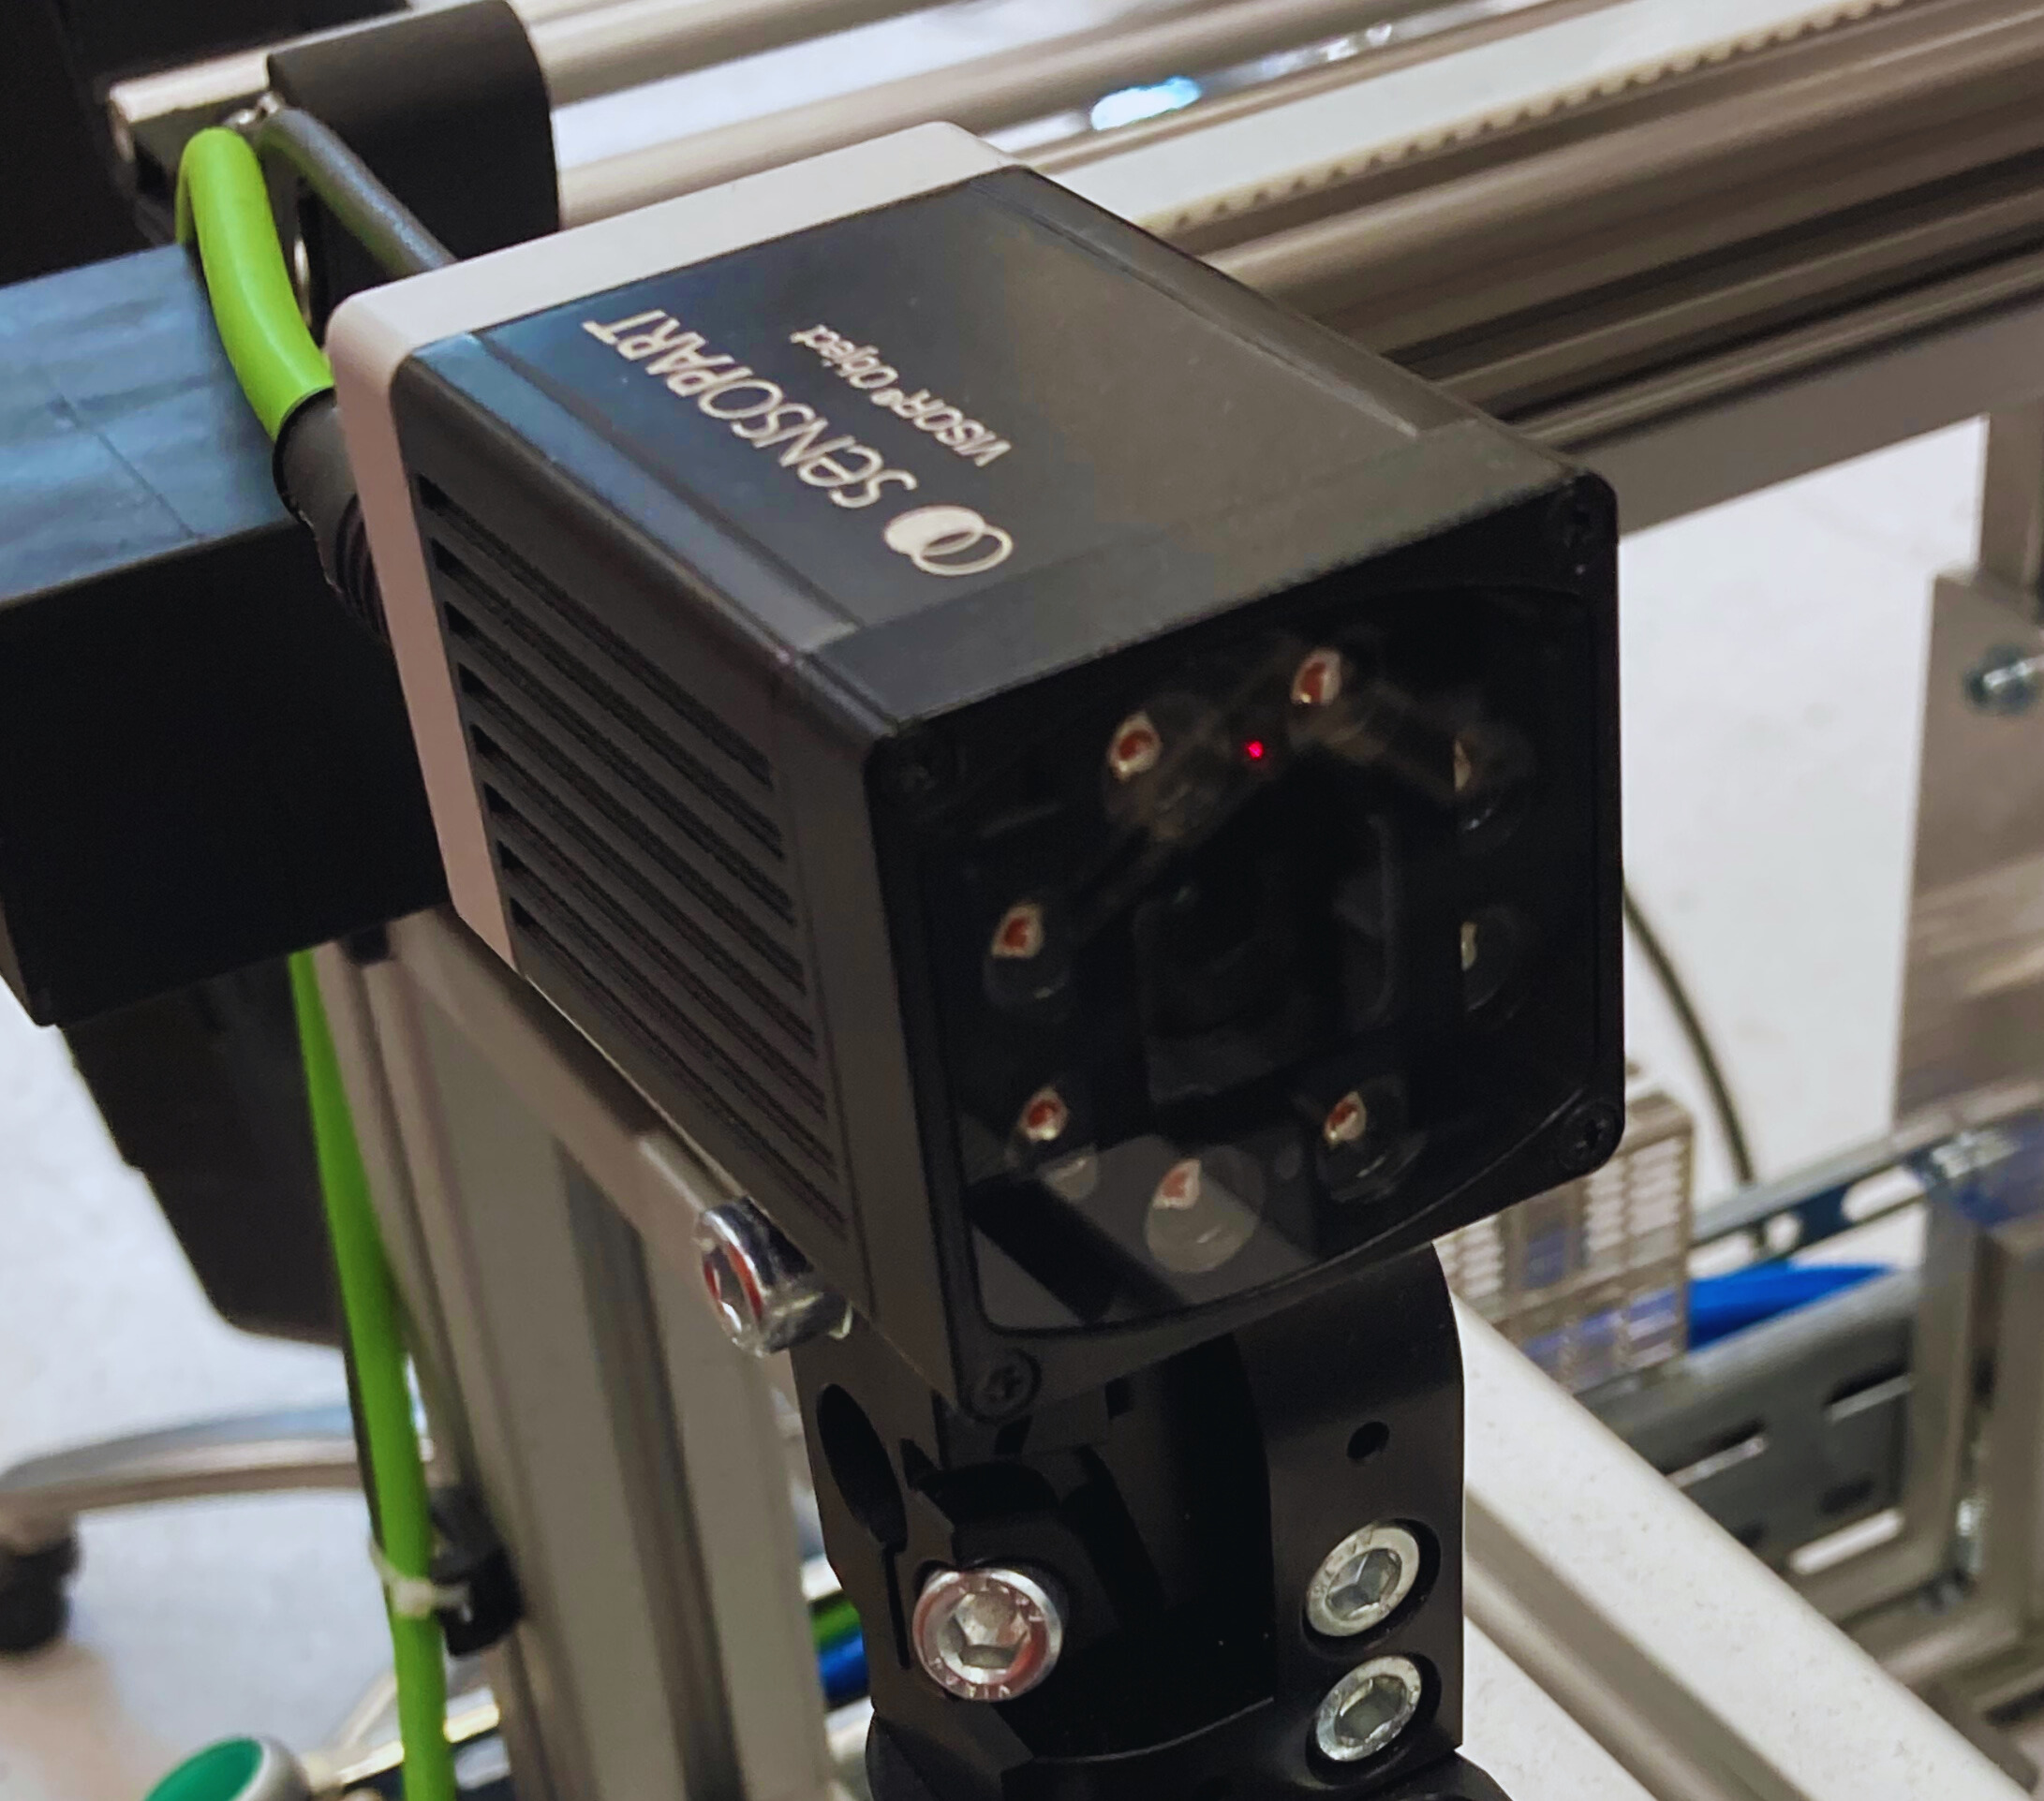
\includegraphics[width=0.5\textwidth]{figures/vision-sensor.png}
    \caption{\hyperref[acro:VISOR]{VISOR}\textsuperscript{\textregistered} vision sensor}
    \label{fig:vision-sensor}
\end{figure}

\begin{table}[h!]
    \centering
    \small
    \renewcommand{\arraystretch}{1.2} % Adjusts row height
    \begin{tabular}{ll}
        \textbf{Description} & \textbf{Value} \\ \hline
        Operating Voltage & 24 V DC (18 V - 30 V) \\
        Startup time & $<$ 14 s\\
        Current consumption & $\leq$ 300 mA \\
        Interfaces & 100 Mbit LAN, PROFINET,\\
        & EtherNet/IP, SensoWeb\\ 
        Weight & Approx. 200 g \\ 
        Ambient air temperature operation & 0$^\circ$C - 50$^\circ$C (80 \% humidity,\\
        & non-condesing) \\ 
        Protection Class & IP 65/IP 67 EN 60529\\
        Housing Material & Die-cast aluminium\\
        Camera type & V20 \\ 
        Number of pixels (H $\times$ V) &s 1440 $\times$ 1080\\
        Sensor size & 1/2.9$^{\prime\prime}$ \\ 
        Pixel size & 3.4 $\mu$m $\times$ 3.45 $\mu$m\\
        Technology & CMOS Mono / Color\\
        Light type & LED Red\\ 
        Target laser & Red, laser class 1\\ 
        Integrated Lens, focal length & 6.5 (Wide)\\
        Focus (Working distance) & Motorized \\ \hline
    \end{tabular}
    \caption{\hyperref[acro:VISOR]{VISOR}\textsuperscript{\textregistered} Technical Data (Robotic and Object Camera)(Source: \cite{visor_user_manual})}
    \label{visor-technical-data}
\end{table}

\hyperref[acro:VISOR]{VISOR}\textsuperscript{\textregistered} vision sensor is a suitable choice for the identification and classification of metal sheets for the automated bending process. These sensors enable precise detection and processing of features on sheet metal parts, which leads to the efficiency and accuracy of automated bending process. The camera can be connected to a PLC or PC through ethernet or profinet. The VISOR software is installed on the PC and then the camera can be configured and jobs can be added.\cite{sensopart-software}. A total of 255 jobs with 255 detectors each can be configured on the camera.

Two camera are selected from SENSOPART. One for the robot which is used to detect the sheet metal parts and the target mark; and the other for inspection jobs.

\begin{figure}[h]
    \centering
    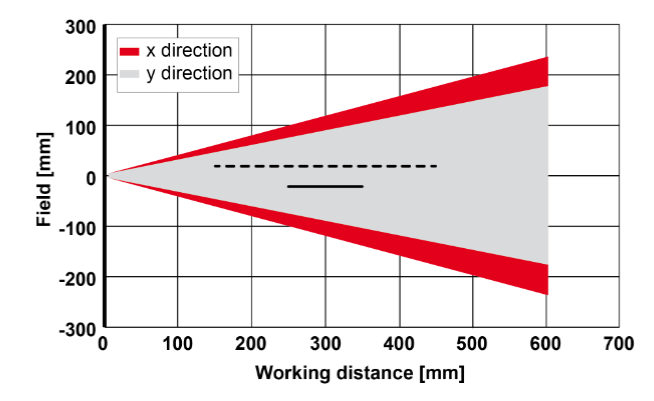
\includegraphics[width=0.75\textwidth]{figures/visor-v20-fov.png}
    \caption{\hyperref[acro:VISOR]{VISOR}\textsuperscript{\textregistered} V20, Field of view Wide, Internal lens (Source: \cite[page 357]{visor_user_manual})}
    \label{fig:visor-v20}
\end{figure}


\subsubsection{Robotic Camera}
\label{subsubsec:robotic-camera}
This camera is a \hyperref[acro:VISOR]{VISOR}\textsuperscript{\textregistered} Robotic V20 vision sensor with $1440 \times 1080$ resolution, wide lens and a red LED light.
\cite{visor-robotic}
A hand-eye calibration is required in order to transform camera poses to robot frame. This camera does not use internal illumination to detect
objects as the working distance is 300.0 mm which is large enough for internal illumination to full brighten the sheet metal part.
A tailored interface is developed for KR teach pendant for this camera to make it communicate with the robot using CBuns.

\subsubsection{Inspection Camera}
\label{subsubsec:inspection-camera}
The inspection camera is a \hyperref[acro:VISOR]{VISOR}\textsuperscript{\textregistered} V20 Object vision sensor with $1440 \times 1080$ resolution and red LED light.
\cite{visor-object}
This camera gets the bending angle
of the bent sheet metal part. The robot brings the bent sheet metal parts to the inspection camera. 
It uses internal illumination of red light to measure the angle as working distance is only around 100 mm. 